%----------------------------------------------------------------------------------------
%	PACKAGES AND OTHER DOCUMENT CONFIGURATIONS
%----------------------------------------------------------------------------------------

\documentclass[a4paper,10pt]{article} 

\usepackage[czech]{babel} % čeština
\usepackage{tabularx}
\usepackage{footnote}

\usepackage{amsmath}
\usepackage{mathtools}
\usepackage{amssymb}
%%\usepackage{matrix}

\usepackage{upgreek} %% stojatá řecká písmena!

\usepackage{fontspec} % fonty
\defaultfontfeatures{Mapping=tex-text}
%\setmainfont{Calibri-Light} % Main document font
%\setmainfont{Lucida Grande}

\usepackage{xunicode,xltxtra,url,parskip} % Formatting packages

\usepackage{fancyhdr}

%\usepackage[usenames,dvipsnames]{xcolor} % Required for specifying custom colors

\usepackage[big]{layaureo} % Margin formatting of the A4 page, an alternative to layaureo
                           % can be \usepackage{fullpage} To reduce the height of the top
                           % margin uncomment:
                           % \addtolength{\voffset}{-1.3cm}
\geometry{left=15mm,right=15mm}

\usepackage{hyperref} % Required for adding links	and customizing them
%\definecolor{linkcolour}{rgb}{0,0.5,0.3} % Link color
%\hypersetup{colorlinks,breaklinks,urlcolor=linkcolour,linkcolor=linkcolour} % Set link colors throughout the document

\usepackage{titlesec} % Used to customize the \section command
\titleformat{\section}{\bf\raggedright}{\thesection.~}{0em}{}
\titlespacing{\section}{0pt}{3pt}{3pt} % Spacing around sections

% PDF settings
\author{Bc. Jan Hladěna}
\hypersetup
{
    pdfauthor={Bc. Jan Hladěna},
    pdfsubject={KNUMA - Zápočtový úkol, sada 2}, 
    pdftitle={KNUMA - Zápočtový úkol, sada 2}
}

\lhead{\textsc{K-AI2-1 KNUMA - Zápočtový úkol, sada 2 - LS 2015/16}}
\rhead{\href{mailto:jan.hladena@uhk.cz}{\textsc{Jan Hladěna}, I1500705}}
\cfoot{}
\renewcommand{\headrulewidth}{0.4pt}
%\renewcommand{\footrulewidth}{0.4pt}

\def\doubleunderline#1{\underline{\underline{#1}}}

\usepackage{chngcntr}

\counterwithin*{equation}{section}
\counterwithin*{equation}{subsection}


\begin{document}
\pagestyle{fancy}

%\font\fb=''[cmr10]'' % Change the font of the \LaTeX command under the skills section

%----------------------------------------------------------------------------------------
% ZÁPOČET
%----------------------------------------------------------------------------------------

\section{Odhadněte graficky polohu kořene dané rovnice a~nalezněte tento kořen metodou
bisekce s~přesností $\upepsilon=10^{-6}$.}

\par Zvoleno zadání a) $x^{2}-cos(x)=0$.
\vfill

%%%% Výpočet

\begin{figure}[!h]
  \begin{center}
    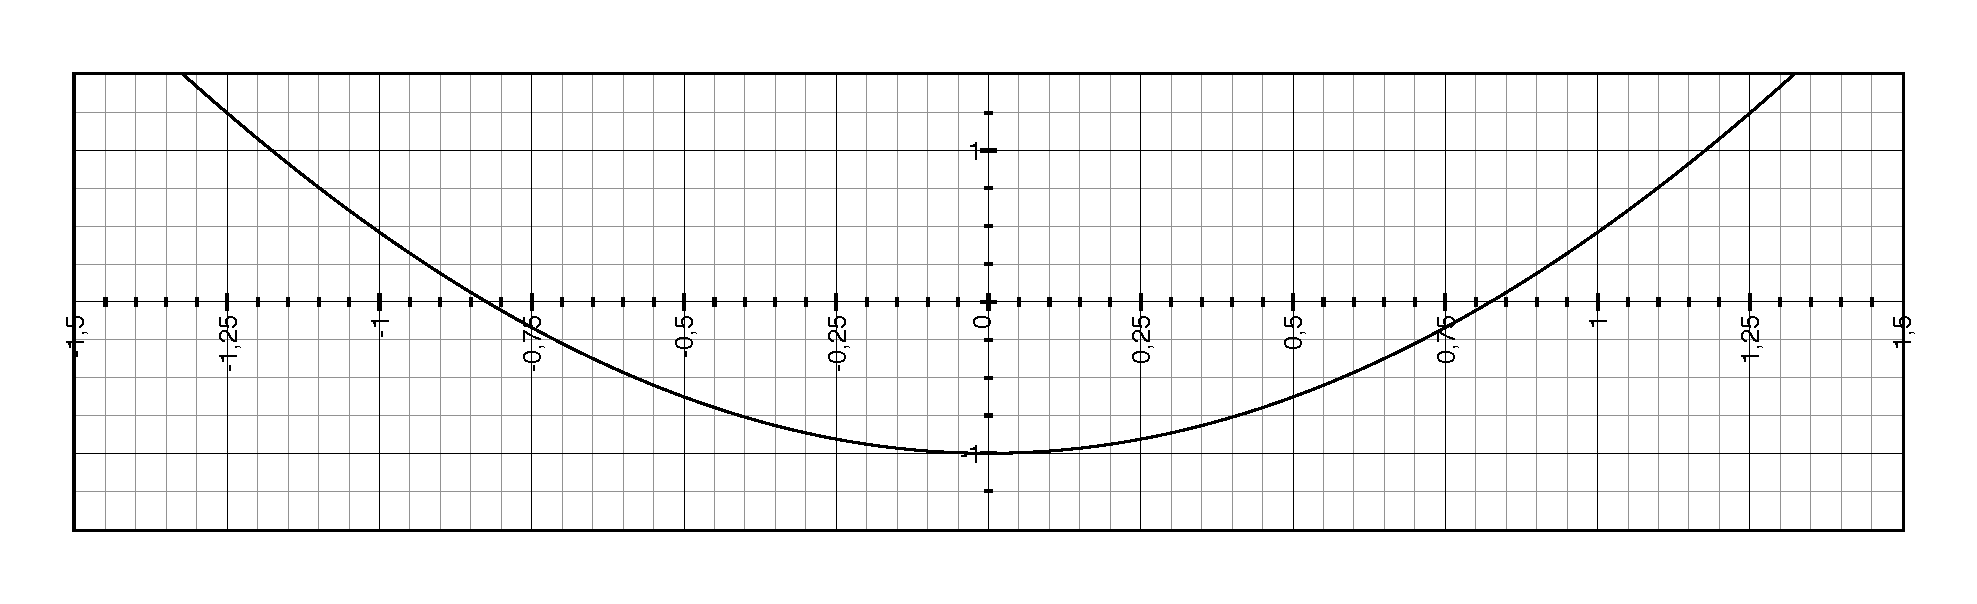
\includegraphics[width=.95\textwidth]{graf1}
  \end{center}
  %\caption{Graf -- $y=x^2-cos(x)$}
\end{figure}

\par Grafický odhad. Funkce představuje symetrickou parabolu ($x^{2}$) posunutou
v~záporném směru osy \emph{y} o~hodnotu určenou goniometrickou funkcí \emph{cosinus}.
Definičním oborem této funkce mohou být všechna reálná čísla. Oborem hodnot funkce je
sjednocení všech kladných reálných čísel parabolické složky $x^{2}$ se~záporným oborem
hodnot funkce \emph{cosinus}, která v~bodě $x=0$ dosahuje svého maxima $y=1$
($-cos(0)=-1$). $D_f:\mathbb{R}$, $H_f:\langle-1; +\infty)$. Parabola protíná osu
\emph{x}~ve~dvou bodech $\upxi_{1}$, $\upxi_{2}$ zrcadlených podle osy~\emph{y}, funkce
má tedy dva reálné kořeny. Pro~odhad bude použito okolí kladného kořene, které bylo
vzhledem k~charakteru růstu jednotlivých složek dané funkce stanoveno
na~$\langle\frac{\uppi}{6}; 1\rangle$.

\par Uvažujme následující program v~prostředí MATLAB využívající rekurzivní funkci
\texttt{bisekce}, přijímající jako argumenty funkci $f\left(x\right)$, hledanou hodnotu
$y$, počáteční meze intervalu $\langle{a}; b\rangle$ a~požadovanou přesnost $\upepsilon$,

\begin{verbatim}
function m = bisekce(funkce, hledana_hodnota, a_start, b_start, epsilon)

% počáteční odhad
m = (a_start + b_start) / 2.0;

% výpočet funkce v bodě odhadu
x = funkce(m);

if (abs(x - hledana_hodnota) >= epsilon)
    % nastaveních nových mezí pro další krok
    if (x - hledana_hodnota < 0)
        a = m;
        b = b_start;
    else 
        a = a_start;
        b = m;
    end
    % rekurze
    m = bisekce(funkce, hledana_hodnota, a, b, epsilon);
end
\end{verbatim}

\par a~její následné zavolání s~odpovídajícimi parametry řešeného příkladu:

\begin{verbatim}
>> xi = bisekce(@(x) x^2 - cos(x), 0, pi/6, 1.0, 10e-6)
xi =

    0.8241
\end{verbatim}

\par Při~požadované přesnosti $\upepsilon=10^{-6}$ budou pak kořeny funkce nalezené
metodou bisekce \doubleunderline{$\upxi_{1,2}=\{-0,824135; 0,824135\}$}.


%----------------------------------------------------------------------------------------
\newpage
\section{Nalezněte všechny kořeny dané rovnice. Použijte Newtonovu metodu. Nejprve vždy
odhadněte polohu kořene a~ověřte Fourierovy podmínky konvergence metody. Kořen hledejte
s~přesností $\upepsilon=10^{-6}$.}

\par Zvoleno zadání b) $\ln{x}+(x+1)^{3}=0$.
\vfill

%%%% Výpočet

\par Funkce je složena z~přirozeného logaritmu a~polynomu třetího stupně. Průnikem
definičních oborů těchto dílčích funkcí $D_{f_{1}}: \{x {\in} \mathbb{R}: x>0\}$,
$D_{f_{2}}:\mathbb{R}$ je obor kladných reálných čísel větších než nula,
$D_{f}: \{x {\in} \mathbb{R}: x>0\}$. Funkce může nabývat hodnot všech reálných čísel,
$H_{f}:\mathbb{R}$. Z~tohoto důvodu lze očekávat pouze jeden reálný kořen, jehož poloha
bude ovlivněna především složkou $\ln{x}$, mající v~nevlastním bodě $x=0$ nevlastní limitu
$\lim_{x=0} \ln{x}=-\infty$ a~protínající osu~\emph{x} v~bodě $x=1$, se~záporným posunem
ve~směru osy~\emph{x} způsobeným složkou kubického polynomu. Odhadovaný interval polohy
kořene $\upxi$ byl tedy zvolen $\upxi \in (0; 0,5\rangle$. \\

\par První derivace: $f'\left(x\right)=\dfrac{1}{x}+3(x+1)^{2}$

\par Druhá derivace: $f''\left(x\right)=-\dfrac{1}{x^{2}}+6(x+1)=-\dfrac{1}{x^{2}}+6x+6$\\

\par Pro~konvergenci Newtonovy metody musí být splněna Fourierova podmínka
$f(x_0){\cdot}f''(x_0)>0$. Jako počáteční aproximace $x_0 \in (0; 0,5\rangle$ byla zvolena
pravá krajní hodnota $x_0=0,5$.

\begin{equation} 
f\left(x_0\right){\cdot}f''\left(x_0\right)>0
\end{equation}

\par Dosazení:

\begin{equation} 
\left(\ln{x_0}+(x_0+1)^{3}\right){\cdot}\left(-\dfrac{1}{x_0^{2}}+6x_{0}+6\right)>0
\end{equation}

\begin{equation} 
\left(\ln{0,5}+(0,5+1)^{3}\right){\cdot}\left(-\dfrac{1}{0,5^{2}}+6{\cdot}0,5+6\right)>0
\end{equation}

\begin{equation} 
\left(\sqrt{e}+1,5^3\right){\cdot}\left(-\dfrac{1}{0,25}+3+6\right)>0
\end{equation}

\begin{equation} 
\frac{-1+0,75+1,5}{0,25}{\cdot}\left(\sqrt{e}+1,5^3\right)>0
\end{equation}

\begin{equation} 
\frac{1,25}{0,25}{\cdot}\left(\sqrt{e}+1,5^3\right)>0
\end{equation}

\begin{equation} 
5{\cdot}(\sqrt{e}+3,375)>0
\end{equation}

\par Fourierova podmínka konvergence pro~počáteční aproximaci $x_0=0,5$ je tedy splněna.
Pro~každý $n$-tý krok výpočtu Newtonovou iterační metodou pak platí

\begin{equation}
x_{n+1}=x_n-\dfrac{f(x_n)}{f'(x_n)}
\end{equation}

Po~dosazení tedy

\begin{equation} 
x_{n+1}=x_n-\dfrac{\ln{x_n}+(x_+1)^{3}}{\dfrac{1}{x_n}+3(x_n+1)^{2}}
\end{equation}

\newpage
\par Obdobně jako v~předchozím příkladě uvažujme následující program v~prostředí MATLAB
s~funkcí \texttt{newton}, přijímající jako argumenty původní funkci $f(x)$, její první
derivaci $f'(x)$, počáteční aproximaci $x_0$ a~požadovanou přesnost $\upepsilon$. Výstupem
funkce je odhad $\upxi$ při~požadované přesnosti $\upepsilon$
a~$n$ označující počet iterací.

\begin{verbatim}
% Newtonova iterační metoda
function [xn, n] = newton(f, df, x0, epsilon)

n = 0;
xk = x0;
xn = x0 - f(x0)/df(x0);

while (abs(xn - xk) > epsilon & n < 250)
    % počítadlo iterací
    n = n+1;

    % aktualizace hodnoty
    xk = xn;
	
    % další člen v řadě
    xn = xk - f(xk)/df(xk);
end
\end{verbatim}

\par Funkce bude bude následně zavolána s~konkrétními argumenty příkladu:

\begin{verbatim}
>> [xi, n] = newton(@(x) log(x)+(x+1)^3, @(x) (1/x)+3*(x+1)^2, 0.5, 10e-6)

xi =
    0.1874    
n =
    3
\end{verbatim}

\par Při~požadované přesnosti $\upepsilon=10^{-6}$ je kořen funkce nalezené Newtonovou
iterační metodou \doubleunderline{$\upxi=0,187439$}.

%----------------------------------------------------------------------------------------
\newpage
\section{Metodou prosté iterace nalezněte všechny kořeny dané rovnice s~přesností
$\upepsilon=10^{-6}$. Nejprve odhadněte polohu kořene (kořenů) a~rovnici upravte
do~vhodného tvaru. Ověřte podmínky konvergence.}

\par Zvoleno zadání b) $f : 5x-8\ln{x}-8=0$.
\vfill

%%%% Výpočet

\par Funkce je tvořena lineárním členem $5x$, absolutním členem $-8$ a~přirozeným
logaritmem $8\ln{x}$. Díky přítomnosti přirozeného logaritmu je definiční obor funkce
$f(x)$ omezen na~kladná reálná čísla větší než nula, $D_{f}: \{x {\in} \mathbb{R}: x>0\}$.


\par Následující tabulka předpokládá existenci dvou kořenů, ležících v~intervalech
$x_{0_2}{\in}{\langle}0,2; 1,5{\rangle}$, resp. $x_{0_1}{\in}{\langle}2,5; 4{\rangle}$.

% fx = @(x) 5*x-8*log(x)-8
\begin{center}
  \begin{tabular}{|c|c|c|c|c|c|}
    \hline
    x & 0,1 & 0,2 & 1,5 & 2,5 & 4,0 \\ \hline\hline
    y & 10,921 & 5,876 & -3,744 & -2,830 & 0,910 \\ \hline
    $sig f(x)$ & $+$ & $+$ & $-$ & $-$ & $+$ \\
    \hline
  \end{tabular}
\end{center}

\par Pro~hledání pevných bodů existují dvě možná ekvivalentní vyjádření funkce $f(x)=0$
ve~tvaru iterační funkce $x=g(x)$:

\begin{equation} 
g_1(x)=\dfrac{8}{5}{\cdot}(\ln{x}+1), \quad g_1'(x)=\dfrac{8}{5}\cdot\dfrac{1}{x},
\quad D_{g_1'}: \mathbb{R}{\setminus}\{0\}
\end{equation}

\begin{equation} 
g_2(x)=\sqrt[8]{e^{5x-8}},
\quad g_2'(x)=\dfrac{5}{8}\cdot\sqrt[8]{e^{5x-8}},
\quad D_{g_2'}: \mathbb{R}
\end{equation}

\par Pro~splnění podmínek konvergence prosté iterační metody musí platit, že je daná
funkce $g(x)$ na~odpovídajícím intervalu $I$ spojitá a~zobrazuje tento interval $I$ zpět
na~tentýž interval $I$. Ověření spojitosti funkce $g(x)$ lze provést důkazem, že v~daném
intervalu $I$ existuje její derivace $g'(x)$, tedy $I{\subset}D_{g'}$. Platí-li zároveň
$|g'(x)|<0, {\forall}x{\in}I$, pak v~tomto intervalu existuje právě jeden pevný bod.

\begin{center}
  \begin{tabular}{|c|c|c|}
    \hline
    $I_{1,2}$ & $I_2=\langle{0,2}; 1,5\rangle$ & $I_1=\langle{2,5}; 4\rangle$ \\ \hline\hline
    
    $I_{1,2}{\subset} D_{g_1'}$ & ano & ano \\ \hline
    $I_{1,2}{\subset} D_{g_2'}$ & ano & ano \\ \hline
    
    ${\forall}x{\in}I_{1,2}: g_1\left(x\right){\in} I_{1,2}$ & ne & ano \\ \hline
    ${\forall}x{\in}I_{1,2}: g_2\left(x\right){\in} I_{1,2}$ & ano & ne \\ 
    
    \hline
  \end{tabular}
\end{center}
% g1 = @(x) (8/5)*(log(x)+1)
% g2 = @(x) exp((5*x-8)/8)

Z~přehledové tabulky podmínek pro~intervaly vyplývá, že prostá iterační metoda použitelná
pro~nalezení odhadů $\upxi_{1,2}$ původní funkce $f(x)$ bude konvergovat v~intervalu
$I_1=\langle{2,5}; 4\rangle$ při~použití ekvivalentní funkce $g_1(x)$ a~v~intervalu
$I_2=\langle{0,2}; 1,5\rangle$ při~použití ekvivalentní funkce $g_2(x)$.

\par Uvažujme následující program v~prostředí MATLAB s~funkcí \texttt{iterace} realizující
výpočet odhadu kořene prostou iterační metodou. Argumenty této funkce jsou ekvivalentní
vyjádření funkce $g\left(x\right)$, počáteční bod odhadu $x_0$ a~požadovaná přesnost
$\upepsilon$. Výstupem funkce je odhad $\upxi$ při~požadované přesnosti $\upepsilon$
a~$n$ označující
počet iterací.

\begin{verbatim}
% Metoda prosté iterace
function [xn, n] = itrace(g, x0, epsilon)

n = 0;
x = x0;
% x = g(x) - pevný bod
xn = g(x);

while (abs(x - xn) && n < 250)
    n = n + 1;
    % další krok
    x = xn;
    xn = g(x);
end
\end{verbatim}

\newpage
\par Zavolání programu pro~funkci $g_1\left(x_{0_1}\right)$ v~bodě
$x_{0_1}=3,5 {\in} \langle{2,5}; 4\rangle$:

% 1. fce
\begin{verbatim}
>> [xi1, n1] = iterace(@(x) (8*log(x)+8)/5, 3.5, 10e-6)

xi1 =
    3.6882
    
n2 =
    12
\end{verbatim}

\par Zavolání programu pro~funkci $g_2\left(x_{0_2}\right)$ v~bodě
$x_{0_2}=0,5 {\in} \langle{0,2}; 1,5\rangle$:

% 2.fce
\begin{verbatim}
>> [xi2, n2] = iterace(@(x) exp((5*x-8)/8), 0.5, 10e-6)

xi2 =
    0.5041
    
n2 =
    5
\end{verbatim}

\par Při~požadované přesnosti $\upepsilon=10^{-6}$ jsou kořeny funkce nalezené prostou
iterační metodou \doubleunderline{$\upxi_{2,1}=\{0,504132; 3,688238\}$}.

%----------------------------------------------------------------------------------------
% KONEC
%----------------------------------------------------------------------------------------

\end{document}
